%
%
\documentclass[10pt,a4paper,oneside]{book}

\usepackage[slovene]{babel}
\usepackage[utf8x]{inputenc}
\usepackage[fleqn]{amsmath}
\usepackage{amsfonts}
\usepackage{amssymb}
\usepackage{makeidx}
\usepackage{graphicx}
\usepackage[x11names, rgb]{xcolor}
\usepackage{tikz}
\usetikzlibrary{automata,snakes,arrows,shapes,decorations.text}

\usepackage{../torstyle}
%torstlye predloge:
%Definicija \Def{}
%Primer \Primer{}
%Prirejen itemize \begin{items}

\begin{document}
\begin{titlepage}
\begin{center}
\ \\[8cm]
{\huge Teoretične osnove računalništva}\\[1.5pt]
{\large Zapiski predavanj 2010/2011}\\[15pt]
{\large \today}
\vfill

\parbox{7.5cm}{
\begin{center}

\includegraphics[width=0.15\textwidth]{../CC}\\[5pt]

This work is licensed under a Creative Commons Attribution-NonCommercial-ShareAlike 3.0 Unported License
\end{center}
}
\end{center}
\end{titlepage}
\tableofcontents

%\newpage
%\section{Notacija}
%\begin{itemize}
%	\item[Množice:] Označimo z velikimi tiskanimi črkami. Podamo jih lahko na naslednje načine\\
%	$ A = \lbrace a_1, a_1, a_3, \ldots \rbrace $ - naštevanje elementov\\
%	$ B = \lbrace n | \ \mbox{pravilo za n} \rbrace \ $ - opis elementov
%\end{itemize}

\pagebreak
\chapter{Uvod}
\section{Chomskyeva hiearhija jezikov}
\begin{center}%?is it too big? :P
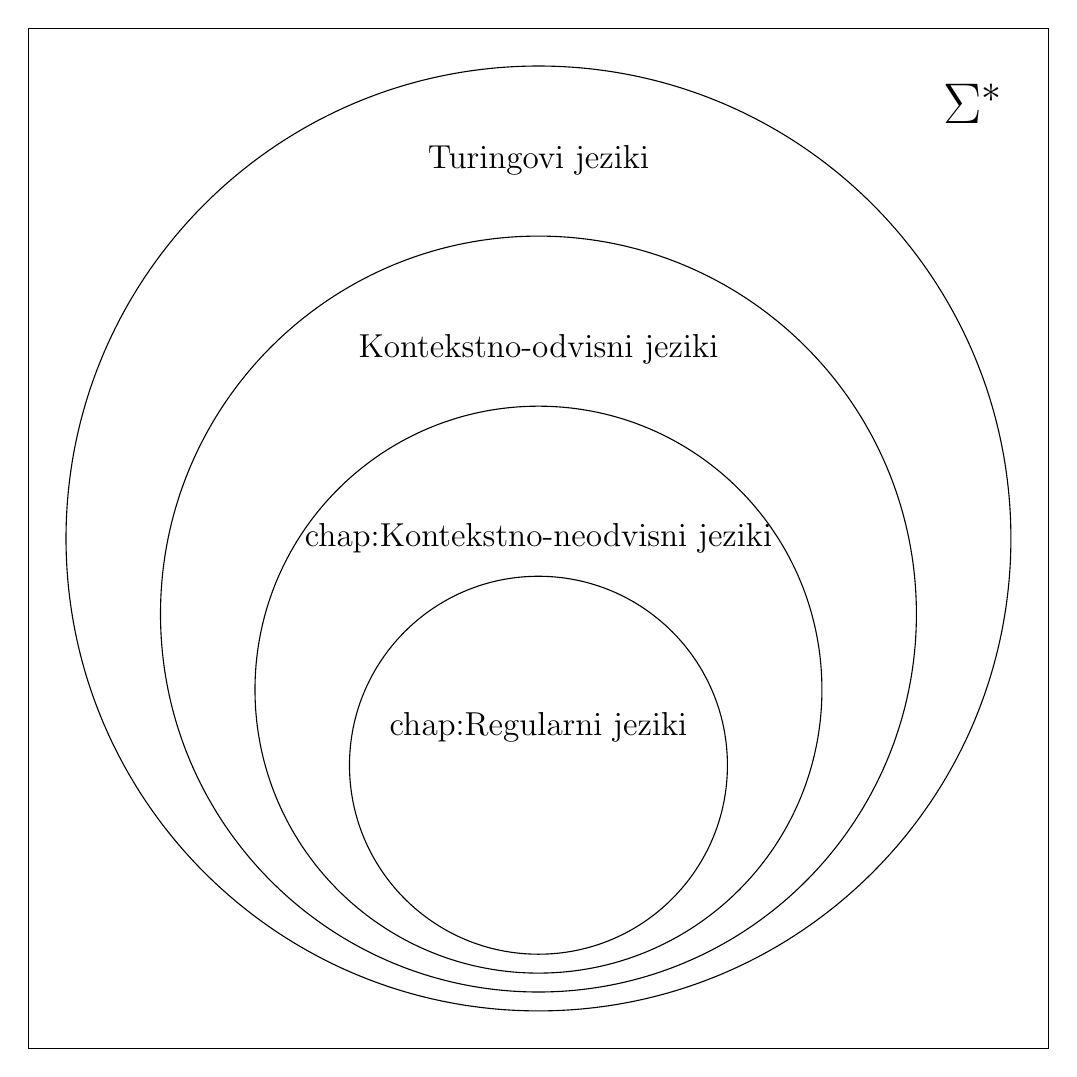
\begin{tikzpicture}[scale=1.2]
	\draw (-5.4cm,-5.4cm) rectangle (5.4cm,5.4cm);
	\node at (4.6cm,4.6cm) {\huge $\Sigma^*$};

	\draw (0cm,0cm) circle (5cm);
	\node at (0,4cm) {\large Turingovi jeziki};%{\nameref{chap:Turingovi jeziki}};

	\draw (0cm,-0.8cm) circle (4cm);
	\node at (0,2cm) {\large Kontekstno-odvisni jeziki};%{\nameref{chap:Kontekstno

	\draw (0cm,-1.6cm) circle (3cm);
	\node at (0,0cm) {\large \nameref{chap:Kontekstno-neodvisni jeziki}};

	\draw (0cm,-2.4cm) circle (2cm);
	\node at (0,-2cm) {\large \nameref{chap:Regularni jeziki}};
\end{tikzpicture}
\end{center}

\section{Matematične osnove}
\subsection{Dokazovanje}
\subsubsection{Dokaz s konstrukcijo}
Dokaz obstoja nekega matematičnega objekta je to, da nam objekt uspe skonstruirati.

\begin{primeri}
\item Za vsak $n>4$, obstaja dvojiško drevo, ki ima natanko $3$ liste.
%?manjka dokaz in slika
\item $| \mathbb{R} | = | [0,1) |$.\\
	\begin{items}
	\item Množici imata enako moč, kadar med njima obstaja bijektivna preslikava.
	\item Vsako realno število $r$ lahko zapišemo kot:
	\begin{displaymath}
		r=\pm d_1 d_2 \cdots d_n . \overline{d_1}\overline{d_2} \cdots \overline{d_m} \cdots;\ d_1 \neq 0
	\end{displaymath}
	\item Definiramo preslikavo:
	\begin{displaymath}
		\mathbb{R}\rightarrow [0,1): r \rightarrow 0.s\overline{d_1} d_{n} \overline{d_2} d_{n-1} \cdots \overline{d_{n-1}} d_2 \overline{d_n} d_1 \overline{d_{n+1}} 0\overline{d_{n+2}} 0 \cdots
	\end{displaymath}
	kjer $s$ določa predznak ($s=0$, če $r \ge 0$ in $s=1$, sicer).
	\item Vidimo:
		\begin{items}
		\item $|\mathbb{R}|\le |[0,1)|$, %?(ker se $0.2$ ne da preslikati v $\mathbb{R}$)??
		\item $|\mathbb{R}|\ge |[0,1)|$, ker velja $[0,1) \subset \mathbb{R}$
		\end{items}
	\item Iz tega lahko sklepamo, da velja $|\mathbb{R}|=|[0,1)|$
	\end{items}
\end{primeri}
	
\subsubsection{Dokaz z indukcijo}
Če je množica induktivni razred%\footnote{Glej slovarček na koncu.}
, lahko z matematično indukcijo dokazujemo neko lastnost članov množice. Induktivni razred $I$ sestavlja:
\begin{items}
\item Baza indukcije - najbolj osnovna množica elementov (osnovni razred)
\item Pravila generiranja - kako iz elementov baze gradimo nove elemente (množico)
\end{items}
\begin{primeri}
\item Induktivni razred naravnih števil $(\mathbb{N})$
	\begin{items}
	\item Baza: $1 \in \mathbb{N}$ 
	\item Pravila generiranja: $n \in \mathbb{N} \Longrightarrow n+1 \in \mathbb{N} $
	\end{items}
\item \fnurl{Hilbertove krivulje}{http://en.wikipedia.org/wiki/Hilbert_curve}
\end{primeri}

\subsubsection{Dokaz s protislovjem}
Vzamemo nasprotno trditev, od tiste, ki jo želimo preveriti in pokažemo, da to vodi v protislovje.

\begin{primeri}
\item Praštevil je končno mnogo.
	\begin{items}
	\item Predpostavimo, da poznamo vsa praštevila:\\
		$P = \{2,3,5,...,p\}$, kjer je $p$ zadnje praštevilo 
	\item Po definiciji obstajajo le praštevila in sestavljena števila (to so taka, ki jih lahko razstavimo na prafaktorje). 
	\item Če pomnožimo vsa znana praštevila iz $P$ in prištejemo $1$ dobimo število, ki se ga ne da razstaviti na prafaktorje iz množice $P$:\\
		$q = 2 * 3 * 5 * ... * p + 1$
	\item Torej je $q$ ali praštevilo (ker ni sestavljeno), ali pa število, sestavljeno iz prafaktorjev, ki jih ni v množici $P$.
	\item Oboje kaže na to, da v množici $P$ nimamo vseh praštevil, ter, da to velja za vsako končno množico praštevil.
	\end{items}
\item $\sqrt[3]{2}$ je racionalno število.
	\begin{items}
	\item Če je $\sqrt[3]{2}$ racionalno število, ga je moč zapisati kot ulomek $\frac{a}{b}$.
	\item Predpostavimo, da je ulomek $\frac{a}{b}$ okrajšan (torej, da velja: $GCD(a,b)=1$):
		\begin{align*}
		\sqrt[3]{2} &= \frac{a}{b}\\
		2 &= \left( \frac{a}{b} \right)^3\\
		2b^3 &= a^3
		\end{align*}
	\item Opazimo, da je $a$ sodo število, torej lahko pišemo $a = 2k$:
		\begin{align*}
		2b &= \left( 2k\right)^3\\
		2b &= 8k\\
		b &= 4k
		\end{align*}
	\item Ker se je pokazalo, da je tudi $b$ sodo število, $GCD(a,b)=1$ ne more držati, torej smo prišli v protislovje in s tem dokazali, da $\sqrt[3]{2}$ ni racionalno število.
	\end{items}
\end{primeri}

\pagebreak
\chapter{Regularni jeziki}\label{chap:Regularni jeziki}

\section{Uvod}
\subsection*{Oznake}
\begin{items}
\item $a$ - simbol (niz dolžine 1)
\item $\Sigma$ - abeceda (končna neprazna množica simbolov)
\item $w$ - niz ali beseda (poljubno končno zaporedje  simbolov $w_1w_2 \ldots w_n$)
\item $|w|$ - dolžina niza
\item $\varepsilon$ - prazen niz, $|w|=0$
\item $\Sigma^*$ - vsi možni nizi abecede
\end{items}

\subsection*{Operacije}
\begin{items}
\item Stik
	\begin{items}
	\item Stik nizov:
		\begin{align*}
		w  &= w_1 w_2 \dots w_n\\
		x  &= x_1 x_2 \dots x_m\\
		wx &= w_1 w_2 \dots w_n x_1 x_2 \dots x_m
		\end{align*}
	\item Stik množic:
		\begin{align*} 
		A & = \lbrace w_1 ,\ w_2 ,\ \dots ,\ w_n \rbrace \\ 
		B & = \lbrace x_1 ,\ x_2 ,\ \dots ,\ x_m \rbrace \\ 
		A \cdot B & = \lbrace w_ix_j \ | \ w_i \in A \ \wedge \ x_i \in B \rbrace
		\end{align*} 
	\end{items}
\item Potenciranje
	\begin{align*} 
	A^0 & = \lbrace \varepsilon \rbrace \\
	A^k & = A \cdot A \cdot \ldots \cdot A \ = \ \bigcirc_{i=1}^{k} A \\
	\end{align*}
\item Iteracija
	\begin{align*} 
	A^* &= A^0 \cup A^1 \cup A^2 \cdots  \ = \ \bigcup_{i=0}^{ \infty } A^i
	\end{align*} 		
\end{items}
\subsection*{Regularni jezik}
\Def{Regularni jezik $L$ nad abecedo $\Sigma$ je poljubna podmnožica $\Sigma^*$
	\begin{equation*} 
	L \subseteq \Sigma^*
	\end{equation*}
}
\begin{primeri} 
\item Prazen jezik: $L_1 =\lbrace \rbrace$
\item Jezik, ki vsebuje $\varepsilon$ (ni prazen): $L_2 = \lbrace \varepsilon \rbrace$
\item Jezik, ki vsebuje nize "a, aa, ab": $L_3 = \lbrace a, aa, ab \rbrace$
\end{primeri} 
\section{Regularni izrazi}\label{sec:RI}
\Def{Osnovni izrazi:
	\begin{items}
	\item $\underline{\emptyset}$ je opisuje prazen jezik $ L(\underline{\emptyset})= \lbrace \rbrace$
	\item $\underline{ \varepsilon }$ opisuje jezik $L(\underline{ \varepsilon })= \lbrace \varepsilon\rbrace$
	\item $\underline{a}$ opisuje jezik $L( \underline{a} ) = \lbrace a \rbrace,\ a \in \Sigma$
	\end{items}
}
\Def{Pravila za generiranje sestavljenih izrazov:
	\begin{items}
	\item $(r_1 + r_2)$ opisuje unijo jezikov $L(r_1 + r_2) = L(r_1) \bigcup L( r_2)$
	\item $(r_1\ r_2)$ opisuje stik jezikov $L(r_1\ r_2) = L(r_1)\cdot L( r_2)$
	\item $(r^*)$ opisuje iteracijo jezika $(L(r))^*$
	\end{items}
}
\begin{primeri}
\item Opiši vse nize, ki se končajo z nizom $00$ v abecedi $\Sigma = \{ 0,1 \}$.
	\begin{displaymath}
	r = (0+1)^*00
	\end{displaymath}
	\item Opiši vse nize, pri katerih so vsi $a$-ji pred $b$-ji in vsi $b$-ji pred $c$-ji v abecedi $\Sigma = \lbrace a,b,c \rbrace$.
		\begin{displaymath}
		a^*b^*c^*
		\end{displaymath}
	\item Opiši vse nize, ki vsebujejo vsaj dva niza '$aa$', ki se ne prekrivata v abecedi $\Sigma = \lbrace a,b,c \rbrace$.
		\begin{displaymath}
		(a+b+c)^* aa (a+b+c)^* aa (a+b+c)^* 
		\end{displaymath}
	\item Opiši vse nize, ki vsebuje vsaj dva niza '$aa$' ki se lahko prekrivata v abecedi $\Sigma = \lbrace a,b,c \rbrace$
		\begin{displaymath}
		(a+b+c)^* aa (a+b+c)^* aa (a+b+c)^* + (a+b+c)^* aaa (a+b+c)^* 
		\end{displaymath}
	\item Opiši vse nize, ki ne vsebujejo niza $11$ v abecedi $\Sigma = \lbrace 0,1 \rbrace$
		\begin{displaymath} 
		(\varepsilon  + 1 )(0^*01)^* 0^*
		\end{displaymath} 
		\begin{displaymath} 
		(\varepsilon  + 1 )(0^* + 01)^*
		\end{displaymath} 
	\item S slovensko abecedo opiši besedo "Ljubljana" v vseh sklonih in vseh mešanicah velikih in malih črk.
		\begin{displaymath}
		(L+l) (J+j) (U+u) (B+b) (L+l) (J+j) (A+a) (N+n) \left( (A+a)(O+o)(E+e)(I+i) \right) 
		\end{displaymath}
		Koliko različnih nizov opišemo s tem regularnim izrazom?\\
		\begin{displaymath}
		2^8 \cdot 2^3 = 2^{11} \mbox{ nizov}
		\end{displaymath}
\end{primeri}
\subsection{Jezik regularnih izrazov}
\Def{Jezik ki ga opisuje poljubni regularni izraz, je regularni jezik.}%?tu bi pasal dokaz ali opis dokaza tega
Regularni jeziki ne vsebujejo informacije o prejšnjih znakih in se z njimi ne da opisati poljubnega jezika. Kasneje bomo za dokazovanje tega uporabljali lemo o napihovanju za regularne jezike (glej \ref{sec:Lema za RJ}).

\begin{primeri}
	%\item $\Sigma^* $ je regularni izraz %?wrong... jezik je nujno strogi subset \sigma*... ker ni dovolj močnega modela za opis vseh možnih nizov
	\item $ \lbrace \rbrace $ je regularni jezik
	\item $ \lbrace 0^n 1^n \ | \ n \geqslant 0 \rbrace $ \underline{ni} regularni jezik%?to bi blo kul pokazat... sam a se da že tuki to?
\end{primeri}

\section{Končni avtomati}\label{sec:KA}
\subsection{Nedeterministični končni avtomati z $\varepsilon$-prehodi }
\Def{$\varepsilon$NKA je definiran kot peterka $M = \langle Q, \Sigma, \delta ,q_0 , F \rangle$, kjer je:
	\begin{items}
	\item $ Q $ - končna množica stanj
	\item $ \Sigma $ - vhodna abeceda
	\item $ \delta $ - funkcija prehodov, $\delta : Q \times (\Sigma \cup \{\varepsilon\}) \rightarrow 2^Q$
	\item $ q_0 $ - začetno stanje
	\item $ F $ - množica končnih stanj
	\end{items}
}
%?razlaga potenčne množice bi šla lahko nekam med mat. osnove... imam še en kup stvari o teoriji množic nekje. Drugač je pa kul - epsilon-closure je že napol opisan :)
$2^Q=P(Q)$ je tu potenčna množica stanj avtomata. To pomeni da je so v $2^Q$ vse možne kombinacije stanj. Recimo da se nahajamo v stanju A, potem nas funkcija prehodov $ \delta $ pripelje v vsa mozna stanja do katerih pridemo iz $A$ z določenim simbolom abecede in z vsemi $ \varepsilon $ prehodi, naprimer $ \lbrace A_1,A2, \ldots , A_n \rbrace$. Tukaj je množica stanj $ \lbrace A_1,A2, \ldots , A_n \rbrace $ element potenčne množice $P(Q)$

\subsection{Nedeterministični končni avtomati}
\Def{NKA je definiran kot peterka $M = \langle Q, \Sigma, \delta, q_0, F \rangle$, kjer je:
	\begin{items}
	\item $ Q $ - končna množica stanj
	\item $ \Sigma $ - vhodna abeceda
	\item $ \delta $ - funkcija prehodov $\delta : Q \times \Sigma \rightarrow 2^{Q}$
	\item $ q_0 $ - začetno stanje
	\item $ F $ - množica končnih stanj
	\end{items}		
}
\subsection{Deterministični končni avtomat}
\Def{DKA je definiran kot petorka $M = \langle Q, \Sigma, \delta, q_0, F \rangle$, kjer je:
	\begin{items}
	\item $ Q $ - končna množica stanj
	\item $ \Sigma $ - vhodna abeceda
	\item $ \delta $ - funkcija prehodov, $\delta : Q \times \Sigma \rightarrow Q$
	\item $ q_0 $ - začetno stanje
	\item $ F $ - množica končnih stanj
	\end{items}	
}

\subsection{Jeziki končnih avtomatov}
\Def{Jezik $\varepsilon$NKA ter NKA je definiran kot:
	\begin{equation*}
	L=\{ w\ |\ \hat\delta(q_0, w) \cap F \neq \emptyset \}
	\end{equation*}
	kjer je $\hat\delta(q,w)$ posplošena funkcija prehodov v večih korakih.}%?Y you no define \varepsilon closure?
\Def{Jezik DKA je definiran kot:
	\begin{equation*}
	L=\{ w\ |\ \delta(q_0, w) \in F \}
	\end{equation*}
}
Definicije želijo povedati, da so v jeziku točno tisti nizi, po katerih je iz začetnega stanja mogoče priti do nekega končnega stanja.

\subsection{Levo in desno-regularne gramatike}\label{sec:LG}
\Def{Regularna gramatika je definirana kot četvorček $G=\langle V,T,P,S \rangle$, kjer je:%?or is it NTPS?
\begin{items}
\item V - množica spremenljivk oz. vmesnih simbolov, $V \subseteq \Sigma$
\item T - množica znakov oz. končnih simbolov, $T \subset \Sigma$
\item P - množica produkcij, $\left[\alpha_1 \rightarrow \alpha_2 \right]$%? se da vse definirat tuki?
\item S - začetni simbol, $S \in V$
\end{items}
Pri tem pa regularne gramatike ločimo na levo in desno-regularne.
\begin{items}
\item Pri levih so produkcije $P \subset V \times ((V \cup \{\varepsilon\})\cdot T^*)$
\item Pri desnih so produkcije $P \subset V \times (T^* \cdot (V \cup \{\varepsilon\}))$
\end{items}
 }
To pomeni, da imamo pri levo-regularnih gramatikah vmesne simbole lahko le na skrajni levi, pri desno-regularnih pa le na desni.

\section{Prevedba med izvedbami regularnih jezikov}%?lame naslov, fixme
Regularni izrazi, regularne gramatike in končni avtomati so vsi enako močni in je mogoče pretvarjati med njimi. V tem odseku bomo predstavili naslednje prevedbe:\\[12pt]%?ustrezno dopolni :)
\begin{center}
\begin{tikzpicture}[>=latex',/tikz/initial text=""]
	\node (RI)   at (0bp,0bp)   {RI};
	\node (eNKA) at (75bp,0bp)  {$\varepsilon$NKA};
	\node (NKA)  at (150bp,0bp) {NKA};
	\node (DKA)  at (225bp,0bp) {DKA};
	\node (DLG)  at (300bp,0bp) {DLG};
	\node (LLG)  at (375bp,0bp) {LLG};

	\draw [bend left,->]  (DKA) to node[auto] {\ref{KA-RI}} (RI);
\end{tikzpicture}
\end{center}

	%nekako tako mam v lanskih vajah, vrjetno mam letos bl prov :)
	%ps. lanske vaje so ful ugly, tko d si nism kj velik pomagov
	%\subsubsection{KA $\rightarrow$ DLG}
	%\subsubsection{DLG $\rightarrow$ KA}
	%\subsubsection{KA $\rightarrow$ RI}
	%\subsubsection{NKA $\rightarrow$ DKA}
	%\subsubsection{$\varepsilon$-NKA $\rightarrow$ NKA}
	%\subsubsection{RI $\rightarrow$ $\varepsilon$-NKA}

\subsection{Končni avtomat $\rightarrow$ Regularni izraz}\label{KA-RI}
Končni avtomat v regularni izraz prevedemo po metodi z eliminacijo. Pri tej metodi izberemo neko vozlišče za eliminacijo, nato pa njegove sosede povežemo med seboj, tako, da na nove povezave zapišemo regularne izraze, ki opisujejo dogajanje v tistem vozlišču. Eliminacijo ponavljamo, dokler nam v avtomatu ne ostanta le dve stanji, nato pa za končni zapis uporabimo naslednji recept:
\br
Na povezavah avtomata imamo zapisane regularne izraze $R,S,Q$ in $T$,\\
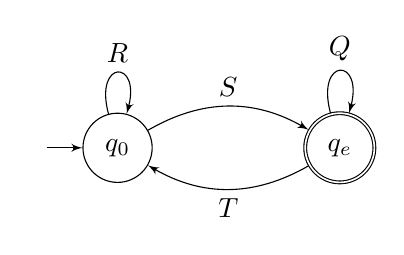
\begin{tikzpicture}[>=latex',/tikz/initial text=""]
	\node (q0) at (0bp,0bp)  [state, initial]   {$q_0$};
	\node (q1) at (80bp,0bp) [state, accepting] {$q_e$};

	\draw [loop above,->] (q0) to node[auto] {$R$} (q0);
	\draw [bend left,->]  (q0) to node[auto] {$S$} (q1);
	\draw [bend left,->]  (q1) to node[auto] {$T$} (q0);
	\draw [loop above,->] (q1) to node[auto] {$Q$} (q1);
\end{tikzpicture}
\\
ki jih prepišemo v en sam regularni izraz oblike:
\begin{displaymath}
(R+SQ^*T)^*SQ^*
\end{displaymath}

\begin{primeri}
\item Zapiši DKA za preverjanje deljivosti s 3 v binarnem sistemu? Zapiši še regularni izraz.\\
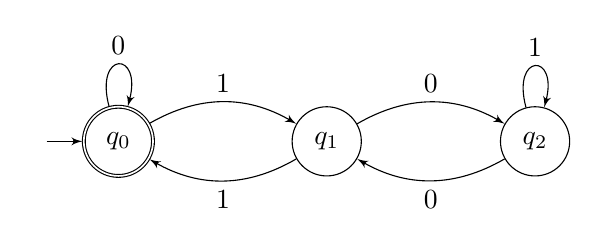
\begin{tikzpicture}[>=latex',/tikz/initial text=""]
	\node (q0) at (0bp,0bp)   [state, initial, accepting] {$q_0$};
	\node (q1) at (75bp,0bp)  [state]                     {$q_1$};
	\node (q2) at (150bp,0bp) [state]                     {$q_2$};

	\draw [loop above,->] (q0) to node[auto] {$0$} (q0);
	\draw [bend left,->]  (q0) to node[auto] {$1$} (q1);
	\draw [bend left,->]  (q1) to node[auto] {$1$} (q0);
	\draw [bend left,->]  (q1) to node[auto] {$0$} (q2);
	\draw [bend left,->]  (q2) to node[auto] {$0$} (q1);
 	\draw [loop above,->] (q2) to node[auto] {$1$} (q2);
\end{tikzpicture}
\ \\
Regularni izraz dobimo po postopku iz \ref{KA-RI}:
\begin{displaymath}
(0+1(01^*0)^*1)^*
\end{displaymath}
\end{primeri}

\section{Ohranjanje regularnosti jezikov}
Regularnost jezika po definiciji ohranjajo operacije:
\begin{items}
\item $L_1 \cup L_2$ - unija 
\item $L_1 \cdot L_2$ - stik 
\item $L^*$ - iteracija
\end{items}
Obstajajo konstruktivni postopki, ki kažejo, da regularnost ohranjajo tudi:
\begin{items}
\item $L_1 \cap L_2$ - presek\\
	Iz avtomatov za $L_1$ in $L_2$ zgradimo t.i. produktni avtomat:
		\begin{align*}
			M_{L_1} &= \{ Q_1, \Sigma, \delta_1, q_{1_0}, F_1 \}\\
			M_{L_2} &= \{ Q_2, \Sigma, \delta_2, q_{2_0}, F_2 \}\\
			M_{L_1}*M_{L_2} &= \{ Q_1 \times Q_2, \Sigma, \delta_*, \langle q_{1_0}, q_{2_0} \rangle, F_1 \times F_2 \}
		\end{align*}
	Namesto stanj dobimo pare stanj in moramo preveriti v kateri par pridemo, če gledamo oba stara avtomata, končna pa so tista stanja, ki so končna v obeh starih avtomatih.
	\begin{displaymath}
		\delta_*(\langle q_1, q_2 \rangle, a) = \langle \delta_1(q_1, a), \delta_2(q_2, a)\rangle
	\end{displaymath}
\item $L^R$ - obrat oz. reverz\\
	Obrnemo vse povezave, ustvarimo novo začetno stanje, ki gre po $\varepsilon$ v stara končna, staro začetno stanje pa postane edino končno stanje.
\end{items}
Regularnost ohranjajo tudi vse operacije, ki so sestavljene iz zgoraj naštetih:
\begin{items}
\item $L_1 \setminus L_2 = L_1 \cap \overline L_2$ - razlika
\item $\overline{L} = \Sigma^* \setminus L$ - komplement
\item $L_1 \underline\vee L_2 = (L_1 \cup L_2) \setminus (L_1 \cap L_2)$ - ekskluzivni ali 
\end{items}

\section{Dokazovanje regularnosti jezika}
%Dostikrat hočemo sestaviti regularen izraz za določen jezik in niti ne vemo ali je regularen izraz sploh regularen ali ne. Za to imamo nekaj metod za dokazovanje regularnosti jezika.%?false... ne moreš sestavit regularnega izraza, ki ni regularen :)
Kadar želimo ugotoviti, ali je nek jezik regularen, to lahko storimo na več načinov:
\begin{items}
\item Pokažemo da je regularen:
	\begin{items}
	\item Jezik skonstruiramo v enem izmed formalizmov, ki sprejemajo regularne jezike:
		\begin{items}
		\item \nameref{sec:KA}
		\item \nameref{sec:RI}
		\item \nameref{sec:LG}
		\end{items}
	\end{items}
\item Dokažemo da ni regularen:
	\begin{items}
	\item Z uporabo leme o napihovanju za regularne jezike (glej \ref{sec:Lema za RJ})
	\item Dokažemo, da jezik ne spada niti v nek širši razred jezikov (recimo, dokažemo, da ni kontekstno-neodvisen)
	\end{items}
\end{items}
%?what is this, I don't even :D
Opozorilo: Če zapišemo regularni izraz za jezik, ali naredimo končni avtomat, moramo dobro preveriti da ne obstaja kakšen protiprimer. Torej beseda ki je v jeziku in jo končni avtomat ali regularni izraz ne sprejme, ali obratno.\\
Če nam ne uspe dokaza (da je ali da ni regularni jezik) do konca speljati, to ne moremo vzeti kot dokaz da ravno nasprotno drži. Velja da v takem primeru še nič ne vemo o regularnosti jezika.

\subsection{Lema o napihovanju za regularne jezike}\label{sec:Lema za RJ}
Lemo o napihovanju za regularne jezike uporabljamo za dokazovanje, da nek jezik ne spada v razred regularnih jezikov. 
\Def{Za vsak regularni jezik obstaja neka konstanta $n$, taka, da lahko vsako besedo $w$ iz jezika, daljšo od $n$, razbijemo na tri dele:
	\begin{displaymath}
	w=u\cdot v\cdot z
	\end{displaymath}
	Pri tem velja:
	\begin{items}
	\item $|uv| \leq n$
	\item $|v| \geq 1$
	\item $uv^iz \in L,\ \forall i \geq 0$ (napihovanje)
	\end{items}
}
Ker dokazujemo da jezik ni regularen, moramo torej najti neko besedo, za katero pri napihovanju ne ostanemo znotraj jezika. Če nam tega z izbrano besedo ne uspe dokazati, še nismo dokazali da je jezik regularen -- edini pravi dokaz tega je konstrukcija jezika v enem izmed regularnih formalizmov.
\br
Če zgornjo definicijo pogledamo v kontekstu končnih avtomatov in vzamemo, da je $n \geq |Q|$, vidimo, da mora v avtomatu obstajati nek cikel, saj sicer tako dolge besede ne bi mogli sprejeti.

\begin{center}
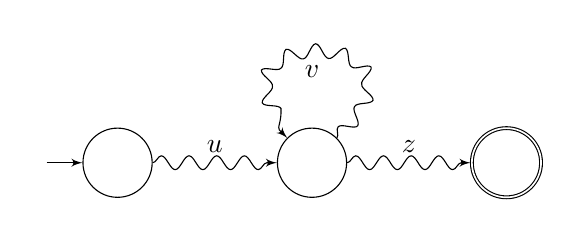
\begin{tikzpicture}[>=latex',/tikz/initial text=""]%scale=0.70, every state/.style={scale=0.70}]
	\node (q0) at (0bp,0bp)  [state, initial]   {};
	\node (q1) at (70bp,0bp) [state]            {};
	\node (q2) at (140bp,0bp) [state, accepting] {};

	\draw [decorate, decoration={snake},->]  (q0) to node[auto] {$u$} (q1);
	\draw [decorate, decoration={snake}, loop,->] (q1) to node[auto] {$v$} (q1);
	\draw [decorate, decoration={snake},->]  (q1) to node[auto] {$z$} (q2);
\end{tikzpicture}
\end{center}

\chapter{Kontekstno-neodvisni jeziki}\label{chap:Kontekstno-neodvisni jeziki}
\section{Kontekstno-neodvisne gramatike}
\section{Skladovni avtomati}
\Def{Skladovni avtomat je definiran kot sedmerka $M=\langle Q, \Sigma, \Gamma, \delta, q_0, Z_0, F \rangle$, kjer je:
	\begin{items}
	\item $ Q $ - končna množica stanj
	\item $ \Sigma $ - vhodna abeceda
	\item $ \Gamma $ - skladovna abeceda
	\item $ \delta $ - funkcija prehodov, $\delta : Q \times (\Sigma \cup \{\varepsilon\}) \times \Gamma \rightarrow 2^{Q \times \Gamma^*}$%? zakaj U \varepsilon?
	\item $ q_0 $ - začetno stanje, $q_0 \in Q$
	\item $ Z_0 $ - začetni skladovni simbol, $Z_0 \in \Gamma$
	\item $ F $ - množica končnih stanj
	\end{items}
}
\subsection{Trenutni opis}
\Def{Trenutni opis je trojka $\langle q, w, \gamma \rangle \in Q \times \Sigma^* \times \Gamma^*$, pri čemer je $q$ trenutno stanje, $w$ preostanek vhodnega niza, ter $\gamma$ trenutna vsebina sklada}
\subsection{Relacija $\vdash$}
\Def{Relacija $\vdash$ nas pelje iz enega trenutnega opisa v drugega, če je ta prehod predviden v funkciji prehodov $\delta$:
	\begin{displaymath}
	\langle q, aw, Z\gamma \rangle \vdash \langle p, w, \gamma'\gamma \rangle \iff \langle p, \gamma' \rangle \in \delta(q,a,Z)
	\end{displaymath}
}
\subsection{Jezik skladovnega avtomata}

%?appendix this:
%\chapter{Slovar}
%?zihr obstaja neki za to, sicer naredi definitions okolje
%\begin{items}
%\item Razred - razred je množica elementov, ki ga lahko podamo z naštevanjem elementov ali z opisom lastnosti (opisni ali konceptualni razredi)
%\end{items}

\end{document}